\section{Research}

\subsection{Music Technology}

\subsubsection{MIDI}

MIDI stands for Musical Instrument Digital Interface, and it is used to communicate music
to computers in separate parts. MIDI files themselves do not contain any audio. Instead, they
send system and channel messages. Each message describes several features, but in this project
we are primarily concerned with note ON/OFF and the timing clock. The note ON/OFF tells which
notes are playing during a certain event and at what velocity. The timing clock keeps track of
when each event is scheduled to occur.

Between these two features we can determine pitch, timing, and expression - the three
components of a note which determine whether or not it is melodic in context.

\subsubsection{DAW}
\label{sec:daw}

DAW stands for Digital Audio Workstation. DAWs are the software that provide an interface
through which users can alter the contents of a MIDI or other audio file. Because our DAW is
to be isolated to a MIDI controller, it  will only contain functions concerning MIDI data.
When dealing with MIDIs, DAWs visualize audio in a piano roll display. The foundation of the
piano roll is a set of rows, each one representing a piano key and its corresponding note.
The horizontal axis represents the timing clock data. For each note that plays in the MIDI, the
piano roll displays a colored bar located in the row of the corresponding note and spanning the
length of the corresponding timing clock data. Additionally, some DAWs show the velocity of the
note by the color of the bar - most commonly, red denotes high velocity while blue/violet
denotes low velocity.

\begin{figure}[h!]
  \centering
  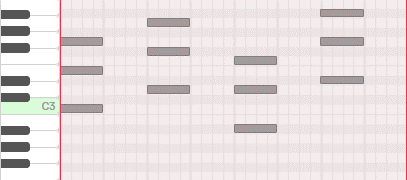
\includegraphics{image/PianoRoll.png}
  \caption{Example of a piano roll display}
  \label{fig:piano_roll}
\end{figure}

The most basic ways a DAW can alter a MIDI are by adding, deleting, and editing notes on the
piano roll; users can change the timing, pitch, and/or velocity of any note. DAWs can also
quantize notes, meaning they will automatically shift the timing of the notes so that every
note begins on some specified fraction of the tempo (most commonly a thirty-second note).
This function is especially useful in adjusting for human errors in timing when writing MIDIs
with a MIDI controller. Better timing makes it easier to synchronize with other tracks that might
end up in the same audio file.


\subsection{AI}

Our original concept for the AI model took a computer vision approach. To begin we would
have had to develop a script which could convert between MIDI data and a PNG
visualization. This image would be similar in structure to what might show on the piano
roll display of a DAW. Each pixel along the vertical axis would represent a key on the
MIDI controller, and each pixel along the horizontal axis would represent some small
fraction of a beat - hypothetically the length of a sixty-forth note, as this is the
shortest common time interval in music. The hue of each pixel would denote the velocity
of the note being played at that time and pitch - a black pixel would mean no note is
being played while a white pixel would show a note being played at maximum velocity.
These images could then be fed into a Convolutional Neural Network (CNN) which would
replicate the visual patterns and thereby output an image that can be converted back into
a MIDI of a completed melody.

\begin{figure}[h!]
  \centering
  
\includegraphics{image/MIDIsample.png}
  \caption{Example of a visualized MIDI file}
  \label{fig:midi_sample}
\end{figure}

This approach was originally considered for its advantages over a more direct MIDI-based
AI. For starters, when conducting some test trials, it was found that the PNG
visualizations are about a quarter the file size of the original MIDIs they were converted
from. This, in conjunction with the comparatively easy calculations of a CNN on a
simplistic bitmap, suggested that a computer vision model would be fast to train.

Additionally, patterns in music are much easier to recognize through visualization than
through note data. Much of the music theory that determines whether a note is melodic in
context is generalized in that it works according to intervals as opposed to discrete
relationships between specific notes. MIDI files don't provide any information about scales
or chords; they simply list which notes were played. It might take an AI a good bit of
to recognize that the interval between C and E is the same as the interval between F and A -
and even longer still to determine which intervals are musically dissonant or not, and in
which contexts. When music is visualized, however, it can generalize the same way it does in
abstract theory. Melodic intervals appear visually the same, regardless of the root note. So
rather than having to learn separately that C pairs well with E and F pairs well with A, it
can generalize that any note will pair well with the note that is four semitones (or in the
AI's case, four pixels) above it, known in music theory as the major third.

The computer vision model was also favored for its level of technical skill. As students, we
have been exposed to the concept of CNNs but have not yet had the opportunity to apply
them. This model felt appropriate for our skill level because it is centered around a
technique we already understand, but it also implements that technique to a degree we have
never attempted before.

\subsubsection{PixelCNN}

For the computer vision model, our lead candidate was PixelCNN. Like a standard CNN,
PixelCNN processes its image inputs an alternating series of masked convolution and pooling.
The "masks" used in the convolution layer are square matrices, and each element of the matrix
is a numerical value that denotes the weight of that element. These masks are iterated over the
input image, convolving with the brightness of the pixels under the mask. In colored images,
the process is repeated once for each color channel: red, green, and blue. Depending on the
configuration of the weights in the matrix, different masks can be used to identify different
visual patterns. Each convolution with each mask outputs a two-dimensional array of values
called a feature map. The feature maps are then put through an activation function, which
modifies the values in the feature map to exaggerate the separation between values above a
certain threshold and  values below it.

Unlike a standard CNN, however, PixelCNN specifically uses masks that only allows it to read
one pixel at a time: row by row, and left to right in each row. This enforces that each pixel
is dependent upon only those above and to the left of itself. Using this unique relationship,
PixelCNN has a unique use-case in predicting the bottom half of an image after processing the
top half as input.

\begin{figure}[h!]
  \centering
  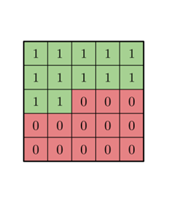
\includegraphics{image/PixelMask.png}
  \caption{PixelCNN's unique mask prevents the AI from peeking ahead}
  \label{fig:pixel_mask}
\end{figure}

This made PixelCNN a particularly appropriate candidate for our computer vision model because
completing an image after processing the first half is exactly the mechanic we planned to use
to achieve the melody autofill. All we would have to do is rotate the input image such that
the time axis propagates top to bottom as opposed to left to right. Additionally, the
dependencies that PixelCNN establishes simulate dependencies in music really well. Whether or
not a note is melodic depends on its context - specifically, the notes that came before it in
time as well as the other notes being played at the same time. Adjusting the axes, PixelCNN's
dependency upon all pixels above equates to the current note being dependent on all notes
that were played before it. As for its left to right dependency, chords are typically built
upward from the root - which, when rotated, would be left to right.

Our main challenge in the use of PixelCNN would be the collection and preprocessing of
training data. For this model to work for our purposes, we would have to convert each MIDI
file into a piano roll visualization which is rotated 90 degrees clockwise.

\subsubsection{Magenta}

\blindtext

\subsection{Embedded Controller Comparisons}
\label{sec:embedded_controllers}

\blindtext

\subsection{DAW Frontend Technologies}

We are looking to use a browser-based frontend Design. This approach is ideal for its ease of
implementing a user interface as well as its cross-platform compatibility. Should we decide to
make the software even more portable by isolating it from the MIDI controller, it will be viewable
on any device that can run a browser. And because of the computational limits of the MIDI
controller, any modern device that is suited for a browser will inherently be able to run the
MIDI autofill software as well.

Our first consideration was React. Considering our group's familiarity with JavaScript as well as
HTML and similar markup languages, it would be easier to work with. However, we ultimately opted to
use Flutter. Flutter's default stylization is sleek and fits in well with the modern aesthetic of
technology. Plus, its widgets allow for more polish on a UI that also has more niche functionality.

As established in \textbf{\ref{sec:daw} \nameref{sec:daw}}, the primary aspect of the UI will be the piano roll display.
The frontend will be responsible for reading the MIDI messages and converting the note ON/OFF and
timing clock features into the position and dimensions of an arbitrary number of UI elements -
each representing a note which can be edited.

\subsection{Raspberry Pi}

As mentioned in \textbf{\ref{sec:embedded_controllers} \nameref{sec:embedded_controllers}}, the Raspberry Pi is mini-computer
which can also function as an embedded controller. The model we're interested in is the
Raspberry Pi 4B. This Raspberry Pi model uses the ARM64 architecture. It can run numerous
ARM64 based Linux distros. The advantage here is the software and tooling that is
available for us to run in a Linux environment. After an analysis of other solutions, we
have decided that the Raspberry Pi is the best fit for our project. To that end, we have
researched how the Raspberry Pi can be configured for use in our project.

\subsubsection{Operating System Choice}

The first configuration choice that needs to be made is the operating system. A Raspberry
Pi out of the box has no operating system. An image must be flashed to an SD card to make
the Raspberry Pi useful. Raspberry Pi's typically run some form of Linux. There are a
number of choices available, as there are many flavors of Linux that can run on the ARM64
architecture. Some common choices for Raspberry Pi include Raspberry Pi OS (formerly known
as Raspian), Arch Linux ARM, and DietPi. Each OS has its advantages and drawbacks, and it
is important for us to select a distro that is well suited for our use case.

The most common operating system used for Raspberry Pi is Raspberry Pi OS. This is a
specially tailored version of Debian for the Raspberry Pi. This is a common choice for any
general purpose usage the Pi. It can be used like a normal desktop computer when a mouse,
keyboard, and monitor are plugged in. This is a "batteries included" distro that includes
many things we will never use. The bloatware from this distro can hinder performance and
waste SD card space. There is a lightweight alternative known as Raspberry Pi OS Lite.
This version does not include any desktop environment.

DietPi is similar to Raspberry Pi OS Lite in that it aims to be a lightweight distro.
DietPi's website claims to be even lighter than Raspberry Pi Os Lite. It occupies 589 Mb
on the SD card, while Raspberry Pi OS occupies 1424 MB. There are a number of other system
optimizations in place to improve general performance. After boot, there are only 11 total
processes, versus 18 total processes running on Raspberry Pi OS.

There are also specialized distros that are only meant to do one specific thing. Examples
include RetroPIE, which is used to run retro video games, or OpenMediaVault, which is used
to turn the device into a networked storage device. This is similar to what we want our
operating system to do. Our use case for the Raspberry Pi is to run one specialized
application that we ourselves develop. It should boot straight into our application with
no other UI from the operating system. The best solution for us is to have a custom distro
just for running our application. Developing a Linux distro from scratch is a difficult
process that is out of the scope of this project. But what we can do is modify an existing
distro to suite our needs.

\subsubsection{Operating System Configuration}
\label{sec:research:subsec:os_config}

The operating system will need to be configured for our use-case. We need to get the
operating system to boot a single GUI application, our DAW, without displaying any other
UI from the desktop environment (DE). There may be more applications separate from the DAW
that will run in the background which also must be started immediately after boot. The
operating system will need to be configured to not permit any networking out of security
and privacy concerns.

To only display a single application, we need to configure the graphics system in our
distro. Graphics in Linux are done through the X Window System. In modern apps, X is
mostly agnostic to the UI, and is used for providing UI toolkits a method for accessing
bitmaps to windows. X can be configured in a variety of ways. The way we intend to
configure X is to host a single fullscreen application for our DAW. This can be done
through the \url{.xinitrc} file. This file specifies which commands to run whenever the X
server is started. By simply including the command to run our application in there, we
will have a single window at startup.

\begin{lstlisting}[language=bash, label={lst:xinitrc}, caption=Example .xinitrc]
#!/bin/sh

exec chromium --kiosk http://127.0.0.1:8080/
\end{lstlisting}

Because our app is browser based, the startup application will be a web browser. In our
case we want to use the Chromium browser, which is the open source variant of Google
Chrome. Chromium has a feature called Kiosk mode, which puts the browser in fullscreen
with no border or frame \autocite{chromiumKioskMode}. This in combination with the xinitrc
file fulfills our requirement of only having a single fullscreen application with no other
UI. This feature can be enabled through the \url{--kiosk} command line flag
\autocite{chromiumKioskMode}. See \nameref{lst:xinitrc} for an example of an xinitrc that
launches chromium in fullscreen mode.

Networking can disabled through the \url{/etc/network/interfaces} config file. This config
file is used to declare all networking interfaces, and the interfaces can be removed by
simply removing all lines declaring a networking interface in that file.

\subsubsection{Packer}

A solution we found for customizing an existing Linux distro is Packer. Packer is a
utility that can take an existing operating system image, modify it, and produce a new
image. Modification is done through provisioners, which exist to perform steps, such as
copying files, running shell commands, setting permissions, etc. Packer relies on builders
to carry out the tasks laid out in a configuration file. The builder we will use is called
packer-builder-arm, which builds ARM images and is suitable for a Raspberry Pi.

We can use our own Packer config file to setup all the tasks described in
\nameref{sec:research:subsec:os_config}. For example, we can use the file provisioner to
copy the \url{.xinitrc} file to the home directory, which is used to configure X11 for our
application.

\subsubsection{Performance}

Performance is always a concern when dealing with constrained embedded hardware. The
Raspberry Pi fares better than microcontrollers you would find in a typical MIDI
controller, but is still performance constrained. Our device needs to be able to run a
machine learning model and a UI application, both of which are computationally expensive
tasks.

\paragraph{Magenta}

Magenta serves as a good baseline for measuring performance of music generating AI.
Magenta ships with two machine learning models: MusicRNN and MusicVAE. We have performance
tested both of these in a demo benchmark program on the Raspberry Pi 4B.

The benchmark program we constructed uses Magenta with JavaScript. We use the Tensorflow
node backend for good CPU performance with Node. When executed, the program initializes
both machine learning models, using checkpoints hosted on Google's servers. The program
measures the time passed in seconds for initialization and music generation time.

The MusicRNN model with the provided pretrained checkpoints has shown good performance
overall when autofilling simple and random melodies, below the 5 second threshold we set
in our goals.

\paragraph{UI} Before spending development time on a browser based DAW, it is important to
verify that Raspberry Pi can even run a browser based DAW with acceptable performance.
Since we have not developed the DAW at this point, we have tested an existing web based
MIDI editor in the Raspberry Pi.

We used an online MIDI editor called signal (\url{https://signal.vercel.app/}) to get a
subjective feel for the performance. The test was ran in the chromium web browser on
Raspberry Pi OS. The performance was acceptable, with a couple things feeling a bit slow
Dragging around notes had a small but noticeable latency between the mouse cursor's
movement and the notes position. There was a small but perceptible amount of time between
double clicking to insert a note and the note showing up on screen.

It should be noted that this app was not explicitly designed to be run on such constrained
hardware. Based on our findings here we are confident that we can develop a browser based
app that has exceptional performance on the Raspberry Pi.


\subsection{Keyboard Design}
